\chapter{System Design}

\section{Requirement spesification} \label{sec:requirements}
The requirements are written as stories inspired from agile methodologies. Instead of attempting to write a complete and detailed description of the system, where all requirements is to be implemented, we have written down a backlog of conceivable requirements and wishes, and implemented them with what we assert to be the most important ones first. Requirements are subject to change, and some have not been implemented either due to time or proving unnecessary during the development phase.

\subsection{Non-functional requirements}
Considering that our goal is for the AnyBoard library to be used by different developers for creating games, as well as further developed and maintained, we wish to lower the threshold and difficulty of using the library, as well as contributing to it.

We believe this is done by creating the library and environment in the following ways:

\textbf{NFR-1, Setup should be simple, for both game developers and developers of AnyBoard} - The first barrier of development is setup of the environment. To minimize this, a developer should ideally have to go through as few as possible steps before he or she can use the library, or contribute to it. This is relevant both to the game developer using AnyBoard as a library to create their own game, as well as a developer that wish to contribute or change the AnyBoard library itself.

We believe a simple setup is important for curious developers to test the library, and for more dedicated developers to take the step and modify it for their own needs.

\textbf{NFR-2, AnyBoard should be provided with a rich set of examples} - A common way of understanding the usefulness and workings of any programming library is looking at simple examples demonstrating the code syntax, function and the effects of using that library. They can work both as a way of marketing the library to game developers, and a way of assisting developers in need of help or a starting point for their own game.

This can be done through publishing the code of complete games built with AnyBoard platform, as well as through small code snippets demonstrating some concrete functionality or even test code.

We believe examples are very important for the adoptation of the AnyBoard library by game developers.

\textbf{NFR-3, The features and functionality of AnyBoard should be tested, and easily available} - Tests should be implemented, so that one can confidently change parts of the code without unknowingly breaking part of the code, as well as providing small examples of library usage.

As a code-base grows in size, the barrier to contribute to the code base increases. There are more classes and functions to be understood before one feels confident. One can often feel uncertain of how changing one part of the code affects the rest of the code base, and in fear of breaking some other functionality unknowingly, refrain from changing anything. 

Having written tests for the functionality of the software, can dramatically lower the fear of unknowingly breaking parts of the code-base, and as such lower the barrier for contributing to the AnyBoard library. It also provides examples of how features are used and expected to work, which complements rich examples as well as documentation.

We believe tests are very important for the further development of the AnyBoard library.

\textbf{NFR-4, AnyBoard must be consistently documented, in an accessible and understandable matter, both for new and experienced developers} - Non-internal elements of the framework (Classes and methods intended to be public) should be well documented. Names, parameters and types of parameters should be easily attainable. 

The larger a code base is, the more complex and harder to understand it usually becomes. By providing good documentation, in form of both in-line coding, auto-complete functionality for editors and online documentation, we lower the time used by both game developers and developers of the library to understand and use the it. 
We believe that providing good documentation is vital for the chances for the library to be used and developed further.

\textbf{NFR-5, AnyBoard should strive to have decoupled code, as to maximize re-usability of different parts, and be independent of other libraries} - Code should be decoupled, so parts can easily be replaced without having cascading effects on other parts of the code base. 

An example of this would be using dependency injection: The token manager for instance will be using some sort of bluetooth communicating capabilities in order to communicate with the token. By passing the bluetooth driver to the AnyBoard TokenManager class upon creation, instead of directly calling the bluetooth drivers we know of, the bluetooth communication libraries will be decoupled from the AnyBoard library. 

Decoupling of code allows changing or replacing parts and dependencies of the our library more easily. 

\subsection{Functional requirements}


\begin{table}
\centering
\caption{Functional requirements for token capabilities}
\label{freq:token}

\begin{tabular}{ | m{1cm} | m{9cm}| m{1.5cm} | }
     & {\bf Functionality}                                                                                                                                                                                                                                                       & {\bf Priority} \\
FT-1 & \emph{As a developer}, I need a token manager that holds all tokens, so I easily can obtain the individual tokens instances from different parts of the code.                                                                                                                    & Low            \\
FT-2 & \emph{As a developer}, I want the token manager to be able to scan for and return active tokens nearby, so I'm not required to have intimate bluetooth knowledge.                                                                                                                & High           \\
FT-3 & \emph{As a developer}, I want to be able to replace the token driver without changing my game code, so I can efficiently test and try different tokens.                                                                                                                          & High           \\
FT-4 & \emph{As a developer}, I want tokens to trigger events upon token-token events or token-constrain events, and allow me to subscribe to this and other events, so I can respond to token interaction. & High         \\
FT-5 & \emph{As a developer}, I want to be able to obtain standard tokens and drivers, so I can quickly create a game without having intimate knowledge of hardware or low-level code.      & High           \\
FT-6 & \emph{As a developer}, I need to be able to test how my game is using tokens and responding to token interactions within a digital interface, and not have to use physical tokens for testing, so I can test more efficiently and develop games with tokens I have not acquired. & Medium \\

FT-7 & \emph{As a developer}, I need to be able to connect simultaiously to at least 4 different tokens. & High 
\end{tabular}
\end{table}

\begin{table}
\centering
\caption{Requirements for graphical interface entities}
\label{freq:graphic}
\begin{tabular}{ | m{1cm} | m{9cm}| m{1.5cm} | }
     & {\bf Functionality}                                                                                                                                                                                                          & {\bf Priority} \\
FG-1 & \emph{As a developer}, I want to be able to create menus and menu items that link to new screens or internet web, so I can create a menu-feature quickly                                                                            & Low            \\
FG-2 & \emph{As a developer}, I want to be able to quickly be able to create a rule-screen from a set of written rules and a FAQ from a set of questions, so I can create this feature quickly. & Low            \\
FG-3 & \emph{As a developer}, I wish to be able to retrieve rules and FAQ from a web page, so I don't have to have duplicate information in case I have a web page.                       & Low           
\end{tabular}
\end{table}

\begin{table}
\centering
\caption{Functional requirements for game entities}
\label{freq:game_entities}
\begin{tabular}{ | m{1cm} | m{9cm}| m{1.5cm} | }
     & {\bf Functionality}                                                                                                                                                                                                                                                                                                     & {\bf Priority} \\
FE-1 & \emph{As a developer}, I want to be able to build on a generic Resource model, so I don't have to spend time implementing interactions such as paying, trading or giving resources between Players and/or the Game.                                                                 & High           \\
FE-2 & \emph{As a developer}, I want to be able to build on a generic Card and Deck model, so I don't have to implement standard usages such as shuffling, drawing, playing.                                                                                                                                                          & High           \\
FE-3 & \emph{As a developer}, I want to be able to build on a generic Player model, that holds a Pawn, has a set of resources, a set of cards, a set of missions, points and  similar, so I don't have to implement those & High           \\
FE-4 & \emph{As a developer}, I want to be able to build on a generic Dice model, so I don't have to spend time implementing interactions such as rolling and returning values from a set of dices. & High           \\
FE-5 & \emph{As a developer}, I want to be able to build on a generic Timer model, so I can create events that happens at a set amount time into the game, or after an event.                                                                                                                                                         & Low            \\
FE-6 & \emph{As a developer}, I want to be able to build on a generic Turn model, so I can quickly specify what goes into each turn of a player.                                                                                                                                                                                      & Medium         \\
FE-7 & \emph{As a developer}, I want to be able to build on a generic Board and Tile model with listeners and triggers, so I can quickly specify where one can go from which tile, their distance, what happens when one steps on a tile without having to create the models from scratch. & High           \\
FE-8 & \emph{As a developer}, I want to be able to log events of different severity, and be able to see them, so I can debug my code and see where something fails                                                                                                                                                                    & High           \\
FE-9 & \emph{As a developer}, I want to be able to assign properties and fields to all my models, so I can create my own concepts and define my own properties on top of the existing models. & High
\end{tabular}
\end{table}

Here we present stories that relate to the hardware tokens and the interaction between those and the software platform.

\subsubsection{Tokens}
The ability for simple interaction with tokens is the main feature of AnyBoard that sets it apart from other game engines. Hence, the requirements relating to this is the main part of the platform. Our requirements are shown in table \ref{freq:token}, and is related to simple scanning, connecting and listening to tokens and its interactions as well as decoupling tokens from game code.

\subsubsection{Graphics}
Board games will include common features, such as menus or rules for games. We wish to provide common entities for quick development of these graphical elements. The requirements relating to this are shown in table \ref{freq:graphic}. 

\subsubsection{Entities}
Table \ref{freq:game_entities} shows the requirements relating to logical board game entities. Hybrid board games will include many of the same entities, which was described in section \ref{sec:boardgames_commonalities}. We believe it could be useful for developers to have these available.

\newpage
\section{Application architecture}
AnyBoard will exist over 3 types main parts, as first shown in figure \ref{fig:high_level_components}. \textbf{Tokens}, such as the AnyBoard pawn, or printer, are the tangible pieces that users can interact with. Tokens talk with the second part, the \textbf{Controller}. The controller is run on a smart device, such as a mobile phone or a tablet. Here, all the logic lies for the game, including the rendering of graphics. The third part is a web based community. This part is conceptual, and will not be implemented in this thesis. The application architecture that we will work on in this thesis, consists therefore of the controller and token part, which is shown in figure \ref{fig:overview_architecture}. 
\begin{figure}[ht]
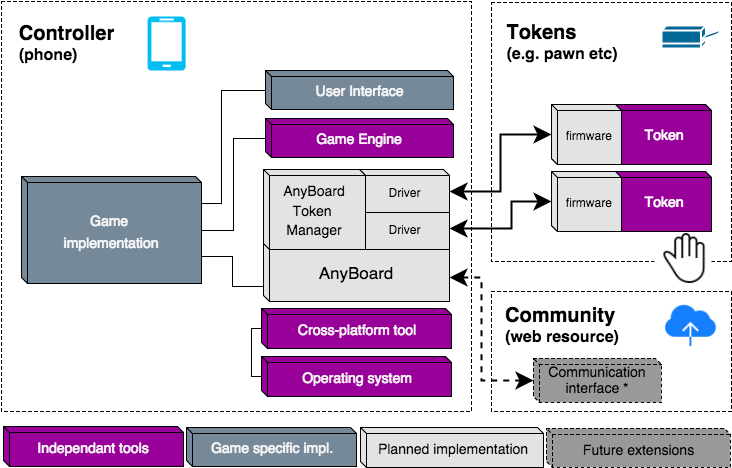
\includegraphics[width=12cm]{img/overview_architecture}
\centering
\caption{Architecture overview. AnyBoard will exist over three components. Tangible tokens such as digital pawns, a game controller/hub running on a smartphone, and an online application assisting the a community of both developers and players. My contribution in this thesis consists of the light grey boxes, denoted "Planned implementation".}
\label{fig:overview_architecture}
\end{figure}

\section{Phone-Token communication}
The means of communicating easily with different tokens is the most central component of AnyBoard. We aim for decoupled token-specific code, to address the requirements in table \ref{freq:token}.

TokenManager is a static component that handles the scanning and connecting/disconnect to tokens.
Its purpose is to identify nearby tokens, and determine an appropriate driver for the token to use. TokenManager has an own driver for this purpose. 

In figure \ref{fig:anypawn_architecture} we see this illustrated. Upon finding suitable drivers for detected tokens, TokenManager instantiates Token A1, Token A2 and Token B. These are Token Class instances, which – seen from the developers point of view – work as a sort of API on top of the tokens. These abstract away the low level communication and commands between AnyBoard and the specific tokens, and provide affordances such as ledOn(), ledOf() and print() functions.

\begin{figure}[ht]
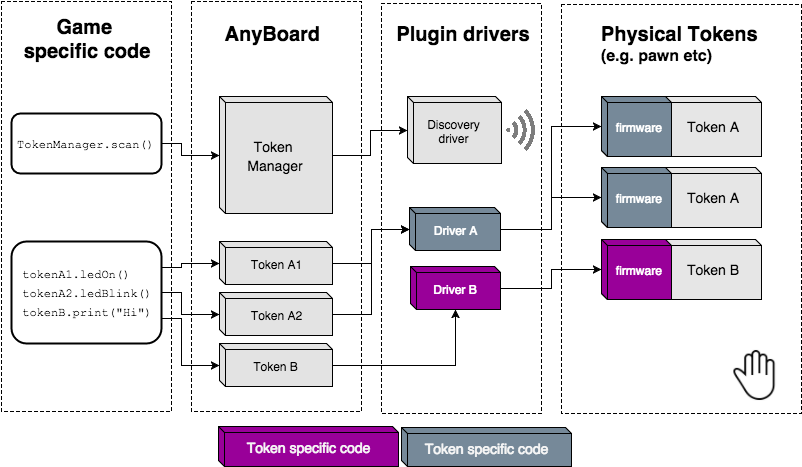
\includegraphics[width=12cm]{img/design_tokenmanager}
\centering
\caption{Communication overview between phone and token. An example where three tokens are discovered by the discovery driver and mapped to two different drivers, which handles the communication with their compatible tokens.}
\label{fig:anypawn_architecture}
\end{figure}


\section{Web-Phone communication}
Web is a component of AnyBoard that will not be implemented in this project, and will hence not be discussed or designed in any detail here. However, it's worth to note some thoughts about this important capability.

We imagine to use HTTP-communication where the phone sends requests to a API on the server. Suggested uses for this communication are:
\begin{enumerate}
\item Retrieving updated FAQ for the game.
\item Sending of events and actions in the game to enable multiplayer functionality, or viewers to watch a game.
\item Sending of events and actions in the game for history/logging.
\item Gathering statistics of usage.
\item Download new games from a Game store
\item Retrieve updates for a current games
\end{enumerate}

The basic tool necessary to enable this sort of communication is capability of communication over the HTTP-protocol. This capability could also be a useful feature for developers that wish to encapsulate web services into their board game or use physical devices that communicate using web APIs. 

This capability is already built into the JavaScript language, with the class XMLRequest. Abstracted HTTP calls using Ajax is also available in a variety of other JavaScript libraries. We therefore see no obstacles for this capability, even without designing for it in the current phase.
\newpage